\documentclass[a4paper,11pt]{article}
\usepackage[utf8]{inputenc}
\usepackage[margin=2.5cm]{geometry}
\usepackage[style=nature]{biblatex}
\addbibresource{cas-refs.bib}
\usepackage{xcolor}
\usepackage{graphicx}
\usepackage{amsmath,amssymb}
\usepackage{amsfonts}
\usepackage[nice]{nicefrac}
\usepackage[title]{appendix}
\usepackage{hyperref}
\usepackage{authblk}
\usepackage[misc]{ifsym}
\usepackage{multirow}
\usepackage{booktabs}
\usepackage{lineno}
\usepackage{float}
\usepackage{comment}


\title{Supplementary Information for Fourier Neural Operators for Accelerating Earthquake Dynamic Rupture Simulations}

\author[$a$]{Napat Tainpakdipat$^1$}
\author[$b$]{Mohamed Abdelmeguid}
\author[$a$]{Chunhui Zhao}
\author[$a,c$]{Ahmed Elbanna}
\affil[$a$]{Department of Civil and Environmental Engineering, University of Illinois Urbana Champaign, Urbana, IL 61801, USA.\vspace{0.05cm}}
\affil[$b$]{Graduate Aerospace Laboratories, California Institute of Technology, Pasadena, CA 91125, USA.\vspace{0.05cm}}
\affil[$c$]{Beckman Institute of Advanced Science and Technology, University of Illinois Urbana Champaign, Urbana, IL 61801, USA.\vspace{0.05cm}\\
\begin{center}
    $^1$E-mail: \href{mailto:napatt2@illinois.edu}{napatt2@illinois.edu}
\end{center}}

\date{}

\begin{document}
\setlength{\parskip}{5pt}
\renewcommand{\thefigure}{S\arabic{figure}}
\renewcommand{\thesection}{S\arabic{section}}

\maketitle

This supplementary information presents examples of predictions from the testing dataset corresponding to selected relative \(L_2\) error and NRMSE values. We present the 2D and 3D dynamic rupture cases in Sections~\ref{sec:supp_2D} and~\ref{sec:supp_3D}, respectively.

\section{2D Dynamic Rupture Predictions}
\label{sec:supp_2D}

This section presents the performance of the FNO-1D model on a testing dataset for 2D dynamic rupture.Figures \ref{fig:2D_mu} - \ref{fig:2D_mu_30std} illustrate testing cases, with the relative \(L_2\) error and the NRMSE reported in each caption serving as quantitative measures of the model’s accuracy. 

\begin{figure}[H]
    \centering
    \includegraphics[width=1 \linewidth]{figures/V2/si/2D/med.png}
    \caption{\label{fig:2D_mu}Testing of the trained FNO-1D model on the 2D dynamic rupture test dataset with a relative \(L_2\) error of 0.0382 and an NRMSE of 0.00227: Panels (a) and (b) show selected input features: (a) initial fractal shear stress distributions \(\tau_{0}\) with \(D=1.5\) and (b) the frictional parameters \(a\) and \(b\), with \(a_0 = 0.007\), \(\Delta a_0 = 0.010\), and \(b=0.012\). Other model inputs (i.e., initial slip rate \(V_0\) with  a threshold \(V_\textbf{th} = 10^{-3}\)~m/s and nucleation stress perturbation \(\Delta \tau\)) are not shown.Panels (c)-(j) show Outputs consist of predicted slip rate snapshots at selected discrete time steps.}
\end{figure}


\begin{figure}[H]
    \centering
    \includegraphics[width=1 \linewidth]{figures/V2/si/2D/med_2mad.png}
    \caption{\label{fig:2D_mu_std}Testing of the trained FNO-1D model on the 2D dynamic rupture test dataset with a relative \(L_2\) error of 0.0456 and an NRMSE of 0.00203: Panels (a) and (b) show selected input features: (a) initial fractal shear stress distributions \(\tau_{0}\) with \(D=1.2\) and (b) the frictional parameters \(a\) and \(b\), with \(a_0 = 0.009\), \(\Delta a_0 = 0.006\), and \(b=0.012\). Other model inputs (i.e., initial slip rate \(V_0\) with  a threshold \(V_\textbf{th} = 10^{-3}\)~m/s and nucleation stress perturbation \(\Delta \tau\)) are not shown.Panels (c)-(j) show Outputs consist of predicted slip rate snapshots at selected discrete time steps.}
\end{figure}

\begin{figure}[H]
    \centering
    \includegraphics[width=1 \linewidth]{figures/V2/si/2D/med_10mad.png}
    \caption{\label{fig:2D_mu_5std}Testing of the trained FNO-1D model on the 2D dynamic rupture test dataset with a relative \(L_2\) error of 0.101 and an NRMSE of 0.00426: Panels (a) and (b) show selected input features: (a) initial fractal shear stress distributions \(\tau_{0}\) with \(D=1.5\) and (b) the frictional parameters \(a\) and \(b\), with \(a_0 = 0.008\), \(\Delta a_0 = 0.008\), and \(b=0.012\). Other model inputs (i.e., initial slip rate \(V_0\) with  a threshold \(V_\textbf{th} = 10^{-3}\)~m/s and nucleation stress perturbation \(\Delta \tau\)) are not shown.Panels (c)-(j) show Outputs consist of predicted slip rate snapshots at selected discrete time steps.}
\end{figure}

\begin{figure}[H]
    \centering
    \includegraphics[width=1 \linewidth]{figures/V2/si/2D/med_15mad.png}
    \caption{\label{fig:2D_mu_8std}Testing of the trained FNO-1D model on the 2D dynamic rupture test dataset with a relative \(L_2\) error of 0.204 and an NRMSE of 0.0107: Panels (a) and (b) show selected input features: (a) initial fractal shear stress distributions \(\tau_{0}\) with \(D=1.5\) and (b) the frictional parameters \(a\) and \(b\), with \(a_0 = 0.0065\), \(\Delta a_0 = 0.011\), and \(b=0.012\). Other model inputs (i.e., initial slip rate \(V_0\) with  a threshold \(V_\textbf{th} = 0\)~m/s and nucleation stress perturbation \(\Delta \tau\)) are not shown.Panels (c)-(j) show Outputs consist of predicted slip rate snapshots at selected discrete time steps.}
\end{figure}

\begin{figure}[H]
    \centering
    \includegraphics[width=1 \linewidth]{figures/V2/si/2D/med_50mad.png}
    \caption{\label{fig:2D_mu_10std}Testing of the trained FNO-1D model on the 2D dynamic rupture test dataset with a relative \(L_2\) error of 0.204 and an NRMSE of 0.0107: Panels (a) and (b) show selected input features: (a) initial fractal shear stress distributions \(\tau_{0}\) with \(D=1.5\) and (b) the frictional parameters \(a\) and \(b\), with \(a_0 = 0.0075\), \(\Delta a_0 = 0.009\), and \(b=0.012\). Other model inputs (i.e., initial slip rate \(V_0\) with  a threshold \(V_\textbf{th} = 0\)~m/s and nucleation stress perturbation \(\Delta \tau\)) are not shown.Panels (c)-(j) show Outputs consist of predicted slip rate snapshots at selected discrete time steps.}
\end{figure}

\begin{figure}[H]
    \centering
    \includegraphics[width=1 \linewidth]{figures/V2/si/2D/med_60mad.png}
    \caption{\label{fig:2D_mu_30std}Testing of the trained FNO-1D model on the 2D dynamic rupture test dataset with a relative \(L_2\) error of 0.204 and an NRMSE of 0.0107: Panels (a) and (b) show selected input features: (a) initial fractal shear stress distributions \(\tau_{0}\) with \(D=1.6\) and (b) the frictional parameters \(a\) and \(b\), with \(a_0 = 0.008\), \(\Delta a_0 = 0.008\), and \(b=0.012\). Other model inputs (i.e., initial slip rate \(V_0\) with  a threshold \(V_\textbf{th} = 0\)~m/s and nucleation stress perturbation \(\Delta \tau\)) are not shown.Panels (c)-(j) show Outputs consist of predicted slip rate snapshots at selected discrete time steps.}
\end{figure}


\section{3D Dynamic Rupture Predictions}
\label{sec:supp_3D}

This section evaluates the FNO-2D model using a testing dataset for 3D dynamic rupture. Figures \ref{fig:3D_mu} - \ref{fig:3D_mu_20std} present various test cases, with each caption detailing relative \(L_2\) error and the NRMSE as quantitative indicators of the model’s accuracy.

\begin{figure}[H]
    \centering
    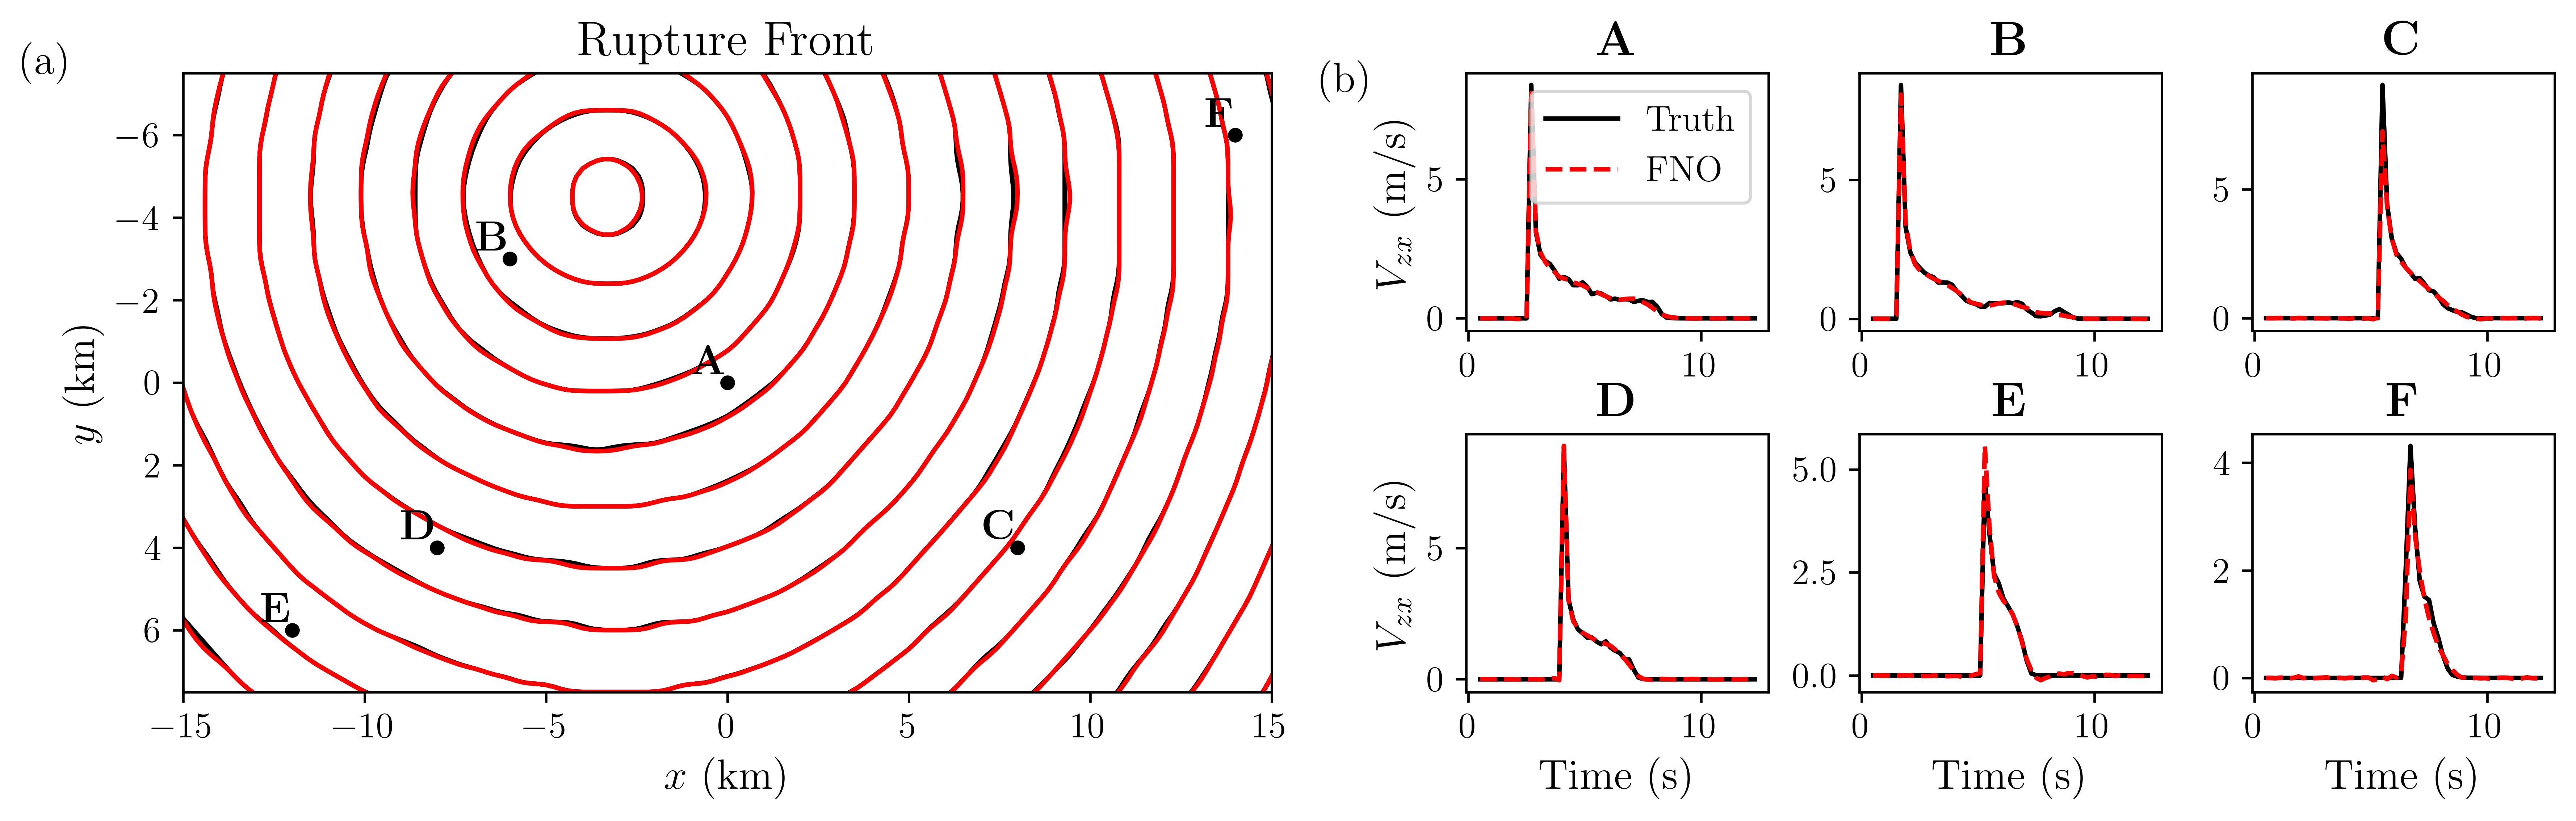
\includegraphics[width=1.0\linewidth]{figures/V2/si/3D/1.png}
    \caption{\label{fig:3D_mu}Results of FNO-2D on the testing dataset for 3D dynamic rupture with a relative \(L_2\) error of 0.100 and an NRMSE of 0.00303. The inputs include the initial fractal shear stress (\(D = 1.6\)); the initial \(V_{zx}\) field (\(V_\text{th} = 10^{-3}\) m/s); a nucleation perturbation; and frictional parameters \(a\) (\(\Delta a_0 = 0.010\), \(a_0 = 0.007\)) and \(b = 0.012\). (a) Rupture front contour plot, showing progression at 0.5 s intervals. (b) Time histories of slip rate at selected points.
    }
\end{figure}

\begin{figure}[H]
    \centering
    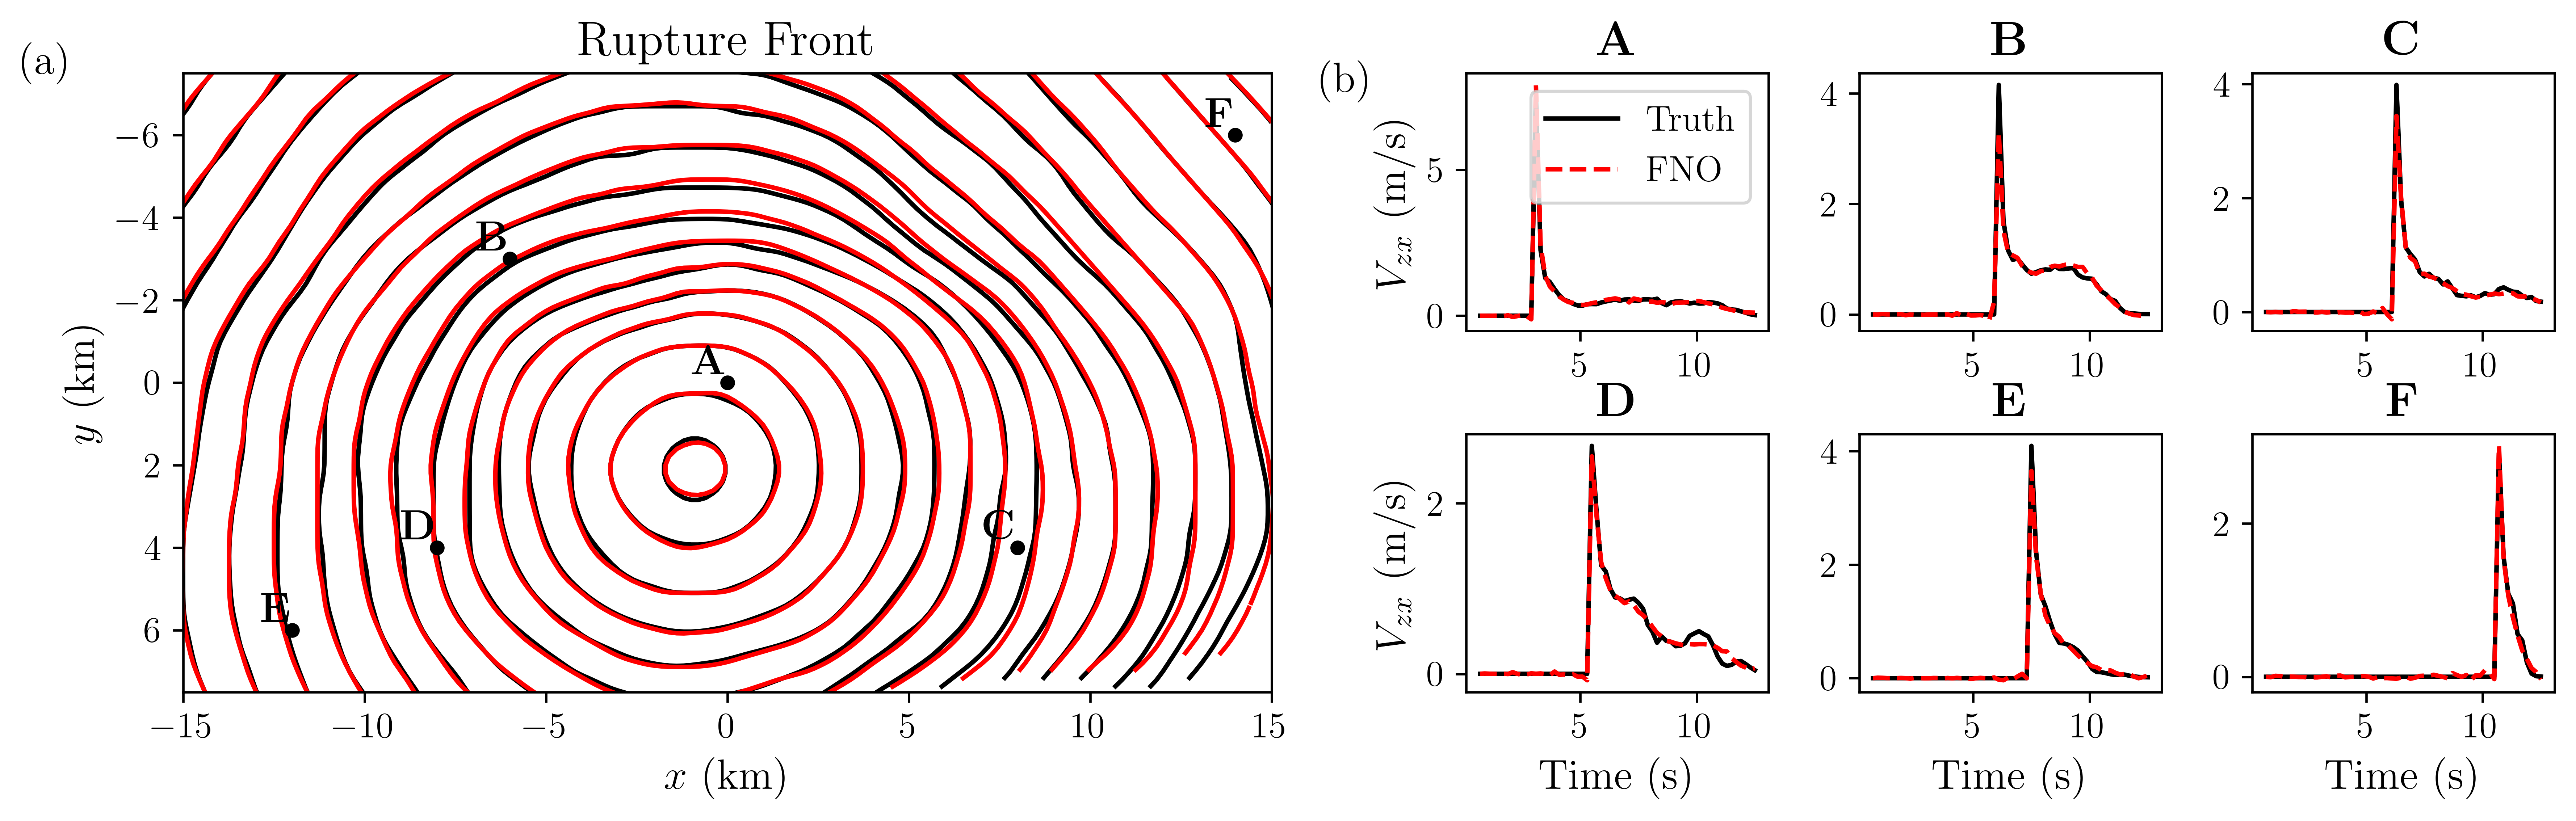
\includegraphics[width=1.0\linewidth]{figures/V2/si/3D/2.png}
    \caption{\label{fig:3D_mu_std}
    Results of FNO-2D on the testing dataset for 3D dynamic rupture with a relative \(L_2\) error of 0.207 and an NRMSE of 0.00587. The inputs include the initial fractal shear stress (\(D = 1.6\)); the initial \(V_{zx}\) field (\(V_\text{th} = 10^{-3}\) m/s); a nucleation perturbation; and frictional parameters \(a\) (\(\Delta a_0 = 0.007\), \(a_0 = 0.0085\)) and \(b = 0.012\). (a) Rupture front contour plot, showing progression at 0.5 s intervals. (b) Time histories of slip rate at selected points.
    }
\end{figure}

\begin{figure}[H]
    \centering
    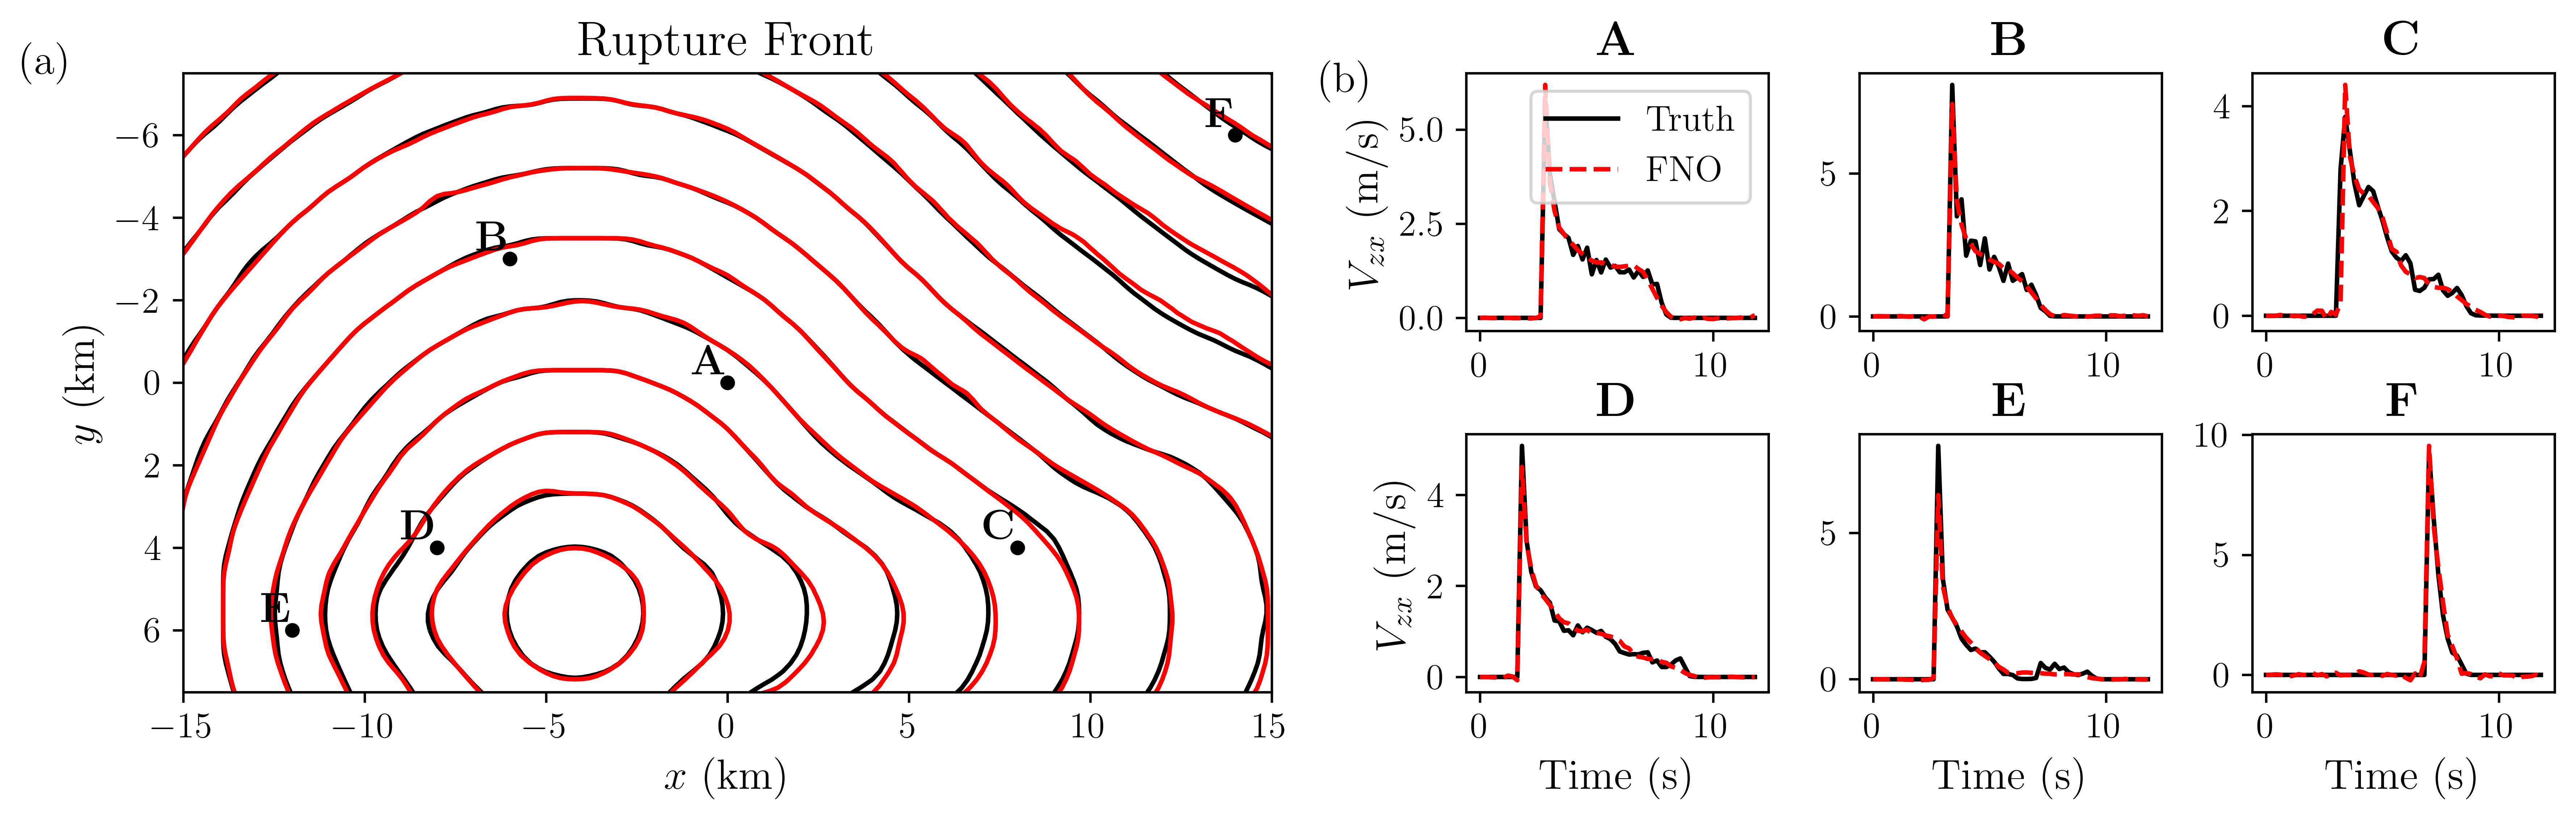
\includegraphics[width=1.0\linewidth]{figures/V2/si/3D/3.png}
    \caption{\label{fig:3D_mu_3std}Results of FNO-2D on the testing dataset for 3D dynamic rupture with a relative \(L_2\) error of 0.306 and an NRMSE of 0.00666. The inputs include the initial fractal shear stress (\(D = 1.5\)); the initial \(V_{zx}\) field (\(V_\text{th} = 0\) m/s); a nucleation perturbation; and frictional parameters \(a\) (\(\Delta a_0 = 0.012\), \(a_0 = 0.006\)) and \(b = 0.014\). (a) Rupture front contour plot, showing progression at 0.5 s intervals. (b) Time histories of slip rate at selected points.
    }
\end{figure}

\begin{figure}[H]
    \centering
    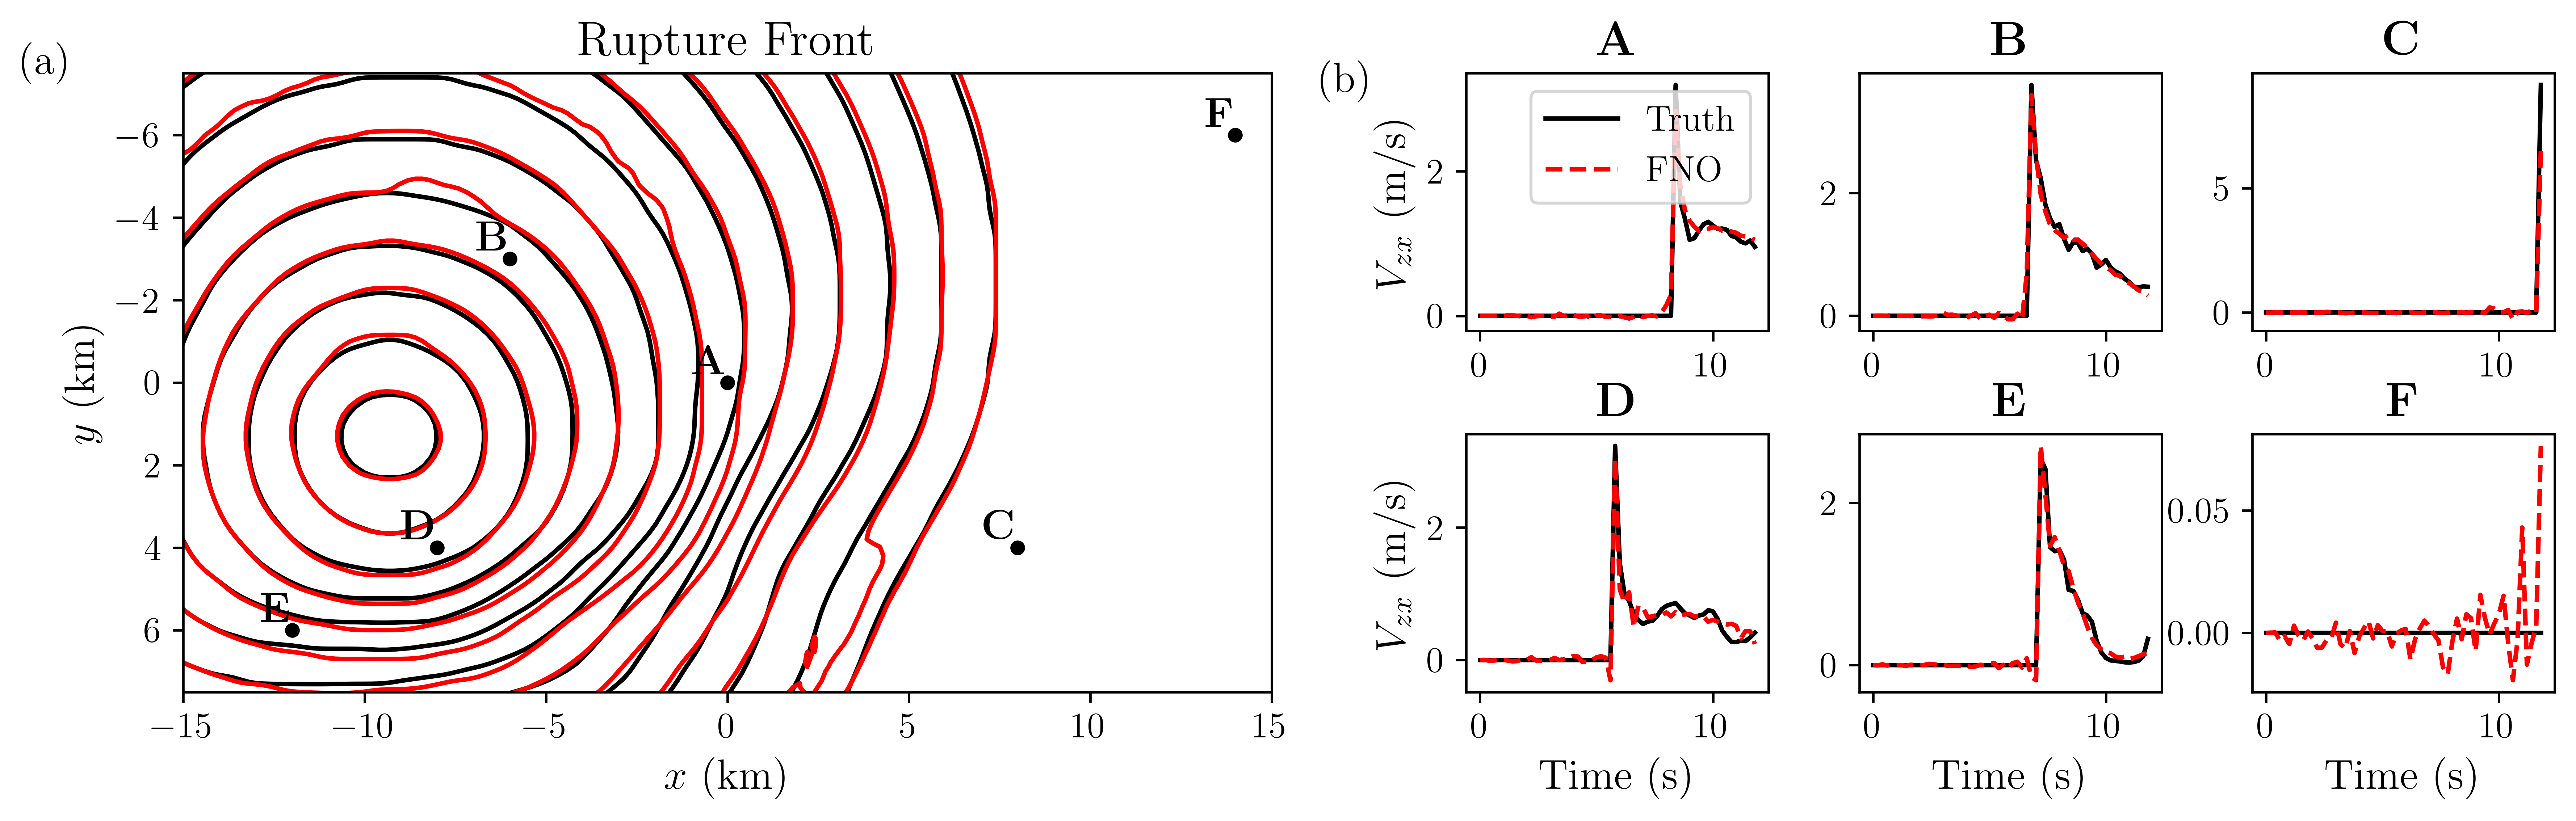
\includegraphics[width=1.0\linewidth]{figures/V2/si/3D/4.png}
    \caption{\label{fig:3D_mu_5std}Results of FNO-2D on the testing dataset for 3D dynamic rupture with a relative \(L_2\) error of 0.403 and an NRMSE of 0.00867. The inputs include the initial fractal shear stress (\(D = 1.2\)); the initial \(V_{zx}\) field (\(V_\text{th} = 0\) m/s); a nucleation perturbation; and frictional parameters \(a\) (\(\Delta a_0 = 0.006\), \(a_0 = 0.009\)) and \(b = 0.014\). (a) Rupture front contour plot, showing progression at 0.5 s intervals. (b) Time histories of slip rate at selected points.
    }
\end{figure}

\begin{figure}[H]
    \centering
    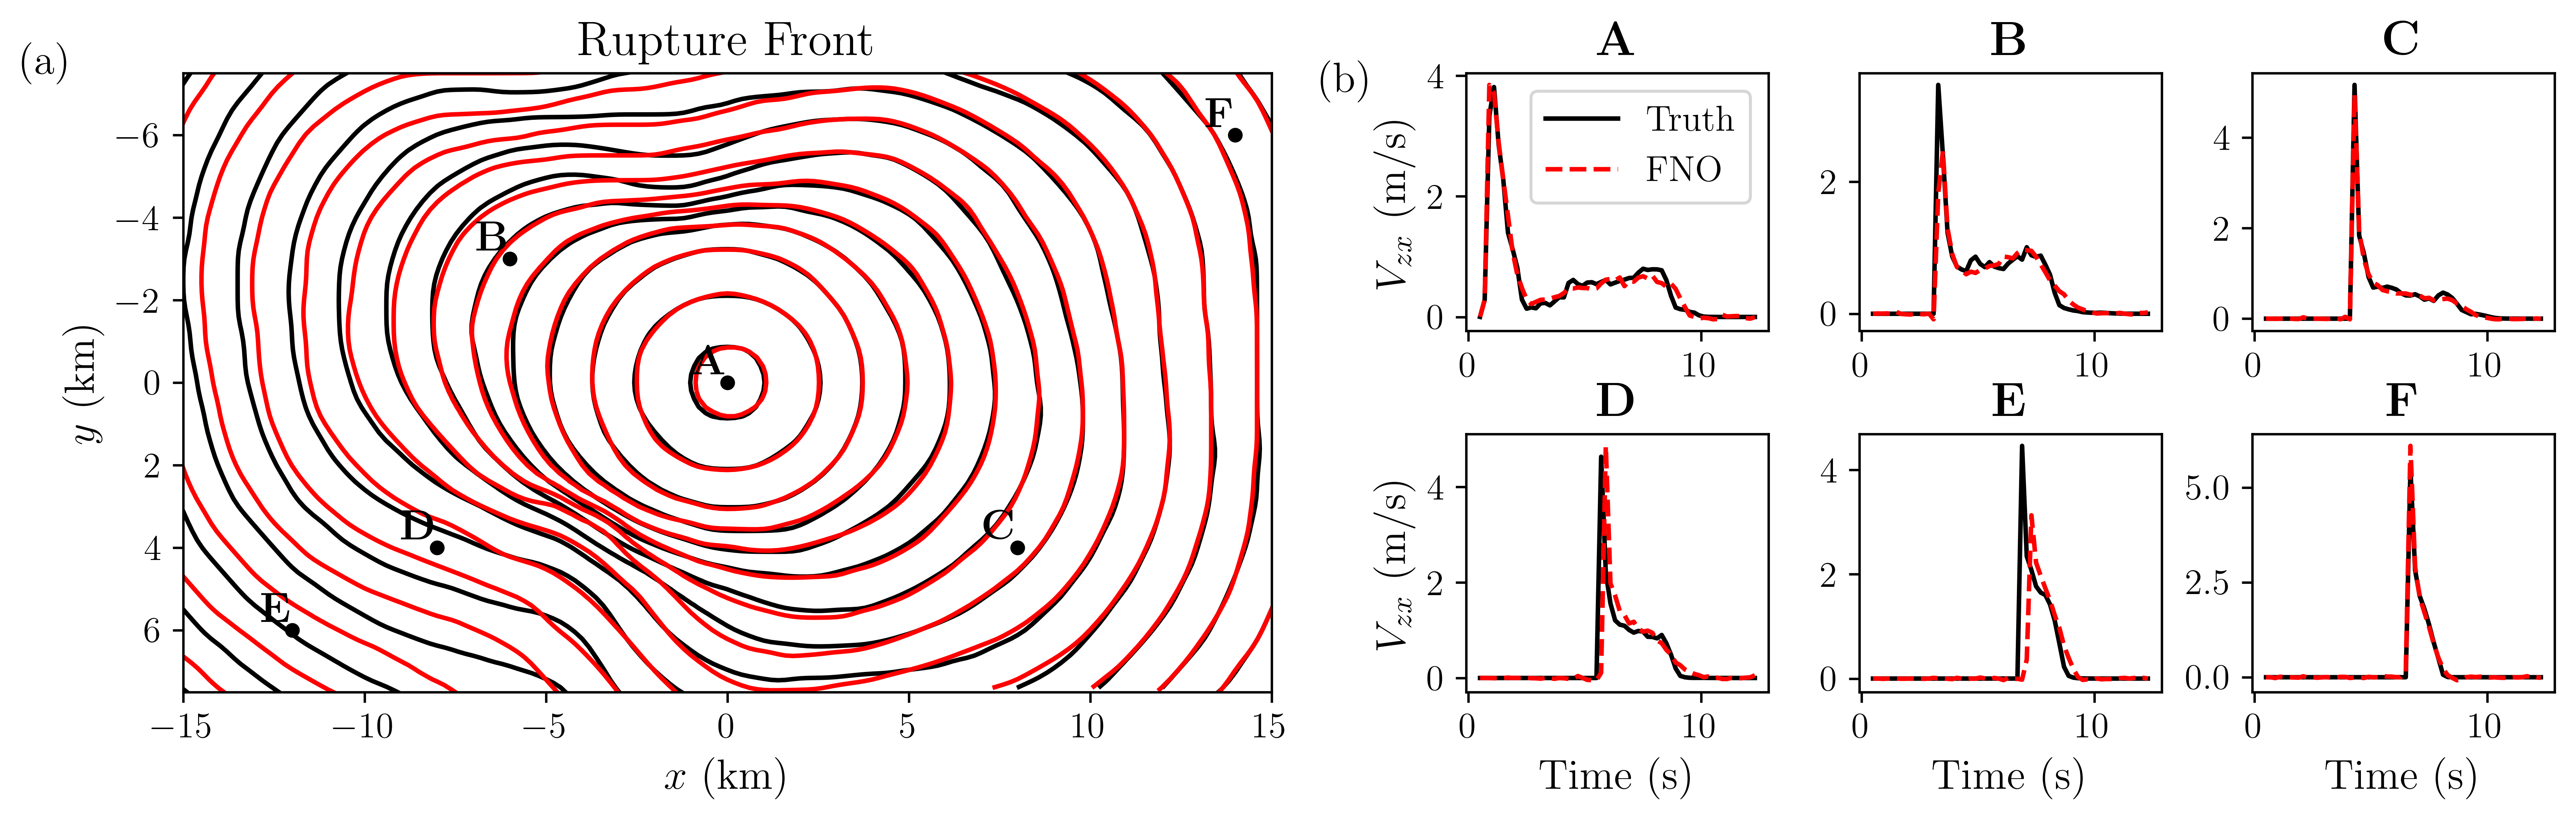
\includegraphics[width=1.0\linewidth]{figures/V2/si/3D/6.png}
    \caption{\label{fig:3D_mu_6std}Results of FNO-2D on the testing dataset for 3D dynamic rupture with a relative \(L_2\) error of 0.631 and an NRMSE of 0.0174. The inputs include the initial fractal shear stress (\(D = 1.5\)); the initial \(V_{zx}\) field (\(V_\text{th} = 10^{-3}\) m/s); a nucleation perturbation; and frictional parameters \(a\) (\(\Delta a_0 = 0.010\), \(a_0 = 0.007\)) and \(b = 0.012\). (a) Rupture front contour plot, showing progression at 0.5 s intervals. (b) Time histories of slip rate at selected points.
    }
\end{figure}


\begin{figure}[H]
    \centering
    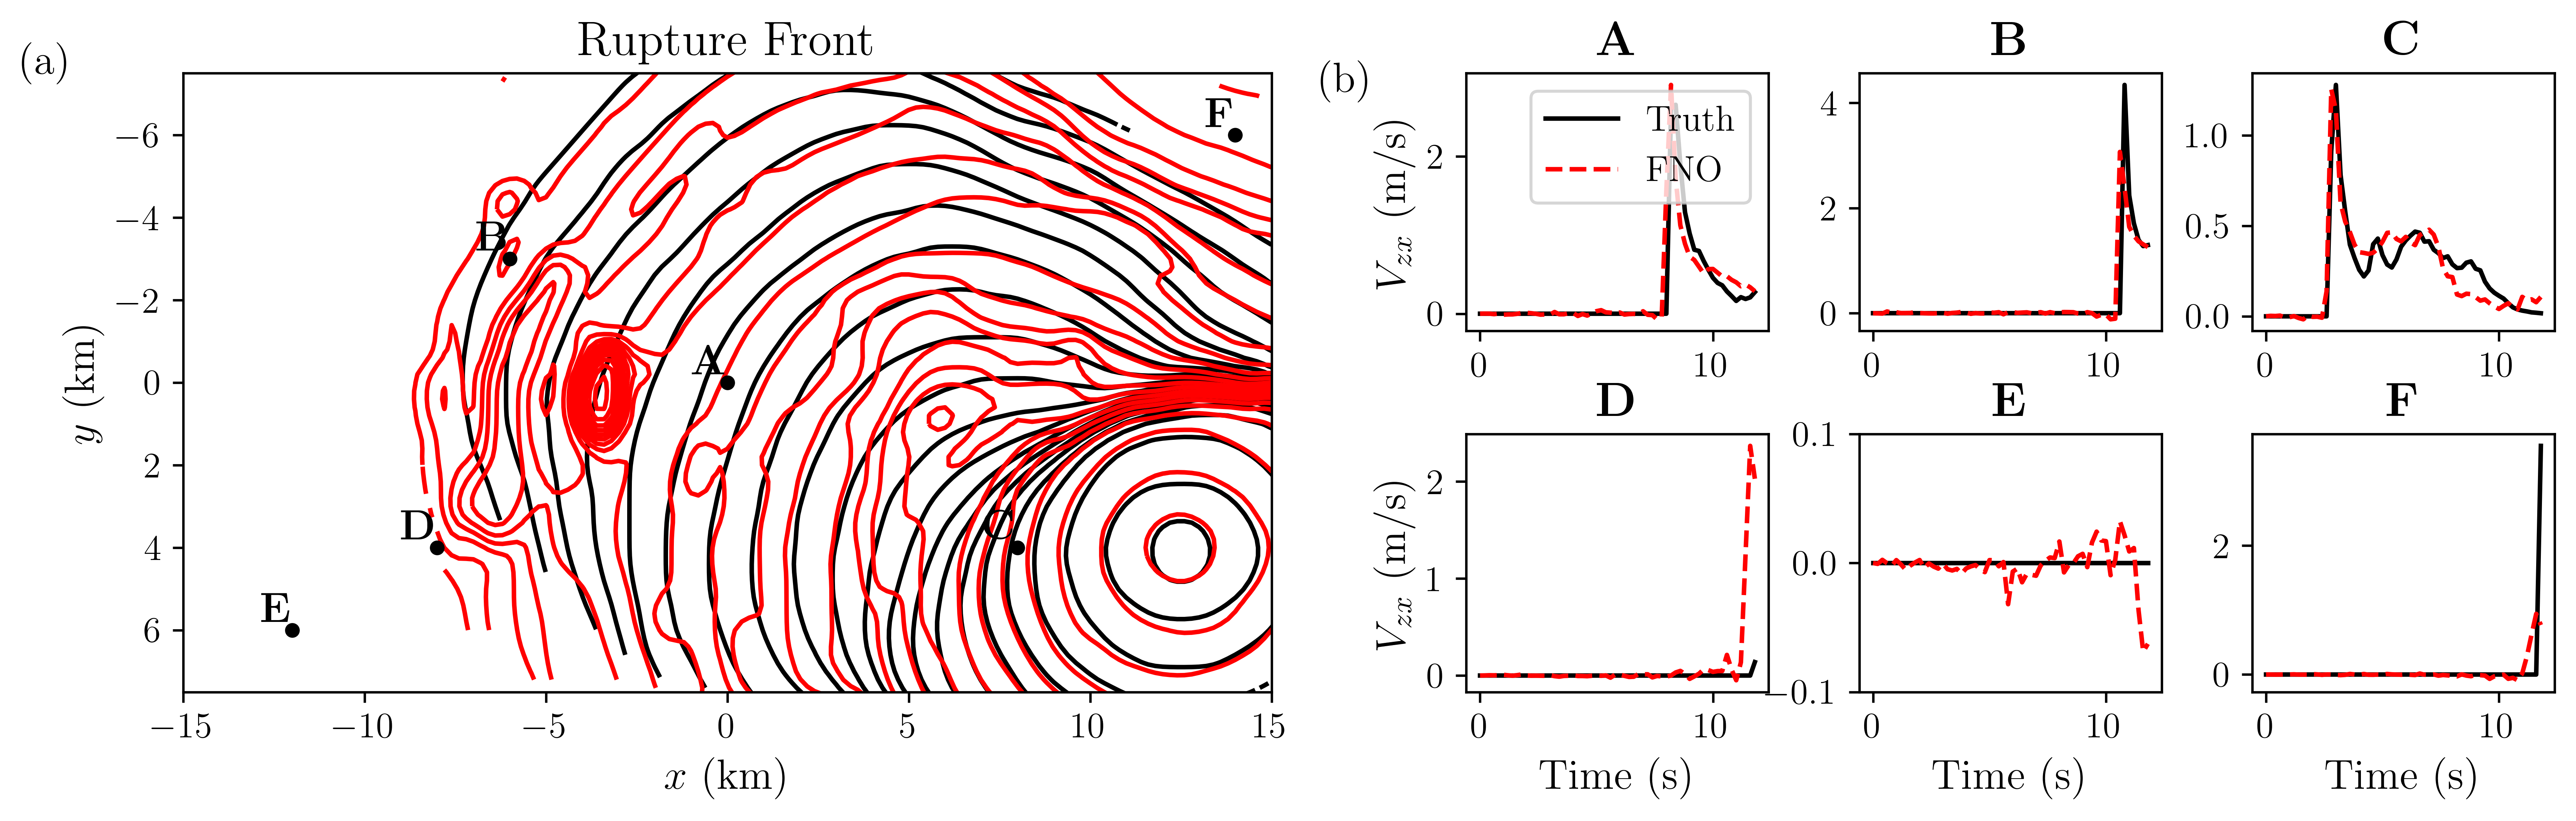
\includegraphics[width=1.0\linewidth]{figures/V2/si/3D/7.png}
    \caption{\label{fig:3D_mu_20std}Results of FNO-2D on the testing dataset for 3D dynamic rupture with a relative \(L_2\) error of 0.807 and an NRMSE of 0.0150. The inputs include the initial fractal shear stress (\(D = 1.2\)); the initial \(V_{zx}\) field (\(V_\text{th} = 0\) m/s); a nucleation perturbation; and frictional parameters \(a\) (\(\Delta a_0 = 0.009\), \(a_0 = 0.0075\)) and \(b = 0.012\). (a) Rupture front contour plot, showing progression at 0.5 s intervals. (b) Time histories of slip rate at selected points.
    }
\end{figure}


\end{document}
